\documentclass[preprint,12pt, a4paper]{elsarticle}
\usepackage{amssymb}
\usepackage{array}
\usepackage{url}

\usepackage{lineno}
% pacotes helon
\usepackage{graphicx}
\usepackage{amsmath}
\usepackage{hyperref}

\graphicspath{{fig/}}

\usepackage{enumerate}

\begin{document}

\begin{frontmatter}

\title{An \textbf{R} library for nonlinear black-box system identification: manual with examples}

\author[pucrio,ppgeps]{Helon Vicente Hultmann Ayala\corref{cor1}}
\ead{helon@puc-rio.br}
\author[ufpr]{Marcos Cesar Gritti}
\ead{cesargritti@gmail.com}
\author[ppgeps,ufpr]{Leandro dos Santos Coelho}
\ead{leandro.coelho@pucpr.br}
\cortext[cor1]{Corresponding author. Tel.: +552135271162; Fax: +552135271165}
\address[pucrio]{Department of Mechanical Engineering, Pontifical Catholic University of Rio de Janeiro (PUC-Rio)\\ Marques de Sao Vicente, 225, Zip code 22453-900, Rio de Janeiro, RJ, Brazil}
\address[ppgeps]{Industrial and Systems Engineering Graduate Program (PPGEPS), Pontifical Catholic University of Parana (PUCPR)\\ Imaculada Conceicao, 1155, Zip code 80215-901, Curitiba, PR, Brazil}
\address[ufpr]{Department of Electrical Engineering, Federal University of Parana (UFPR)\\ Cel. Francisco Heraclito dos Santos, 100, Zip code 81531-980 Curitiba, PR, Brazil}

\begin{abstract}
	In the present manual we provide installation instructions, working examples with code, and the outputs using the \textbf{narmax} toolbox. The raw codes of the examples depicted in this manual can be found in \url{https://github.com/helonayala/narmax/examples}. The example data are real-world acquired data which are freely available in the internet, which facilitates reproduction using concrete real-world examples. 
\end{abstract}

\end{frontmatter}

\section{Installation}

The package code is attached to the paper in a zip file. It has been tested on the cloud in the freely available service \url{https://rstudio.cloud/}. The following steps should be made to install the package and run the examples.
\begin{enumerate}[Step 1:]
	\item \textbf{Prepare the environment}: Install package dependencies and devtools updated version.
	
	\verb|R> install.packages(c("devtools","stringr","latex2exp","ggplot2",|
	\verb|	+ "progress","roxygen2","tidyr"))|
	
	\verb|R> devtools::install_github("r-lib/devtools")|
	
	\item \textbf{Open the project}: Simply click on the \verb|narmax.Rproj| file to open the project file so the environment is configured to build the package.
	
	\item \textbf{Build the package}: Hit CTRL + SHIFT + D to build the documentation and CTRL + SHIFT + B to build the package (in Mac OS, hit use instead of CTRL). If successful the package functions will be available after a \verb|library(narmax)| call.
	
	\item \textbf{Navigate the examples}: To run the examples detailed in the next Section, simply navigate to the \verb|examples/| folder, \textbf{set it as the working directory} (otherwise the filename extensions for reading the data wont't work), and source the desired files.		
\end{enumerate}

The package can be downloaded on the internet, please check GitHub for the most recent version:

\url{https://github.com/helonayala/narmax}

\section{Dowloading the data}  \label{sec:examples}

In order to run the examples, the users should firstly download the third-party data that is freely available on the internet and then dump them in the \verb|data/| folder  

\begin{itemize}
	\item Example 2: click on the link below to download it 
	
	\url{ftp://ftp.esat.kuleuven.be/pub/SISTA/data/thermic/heating_system.dat.gz}
	
	Description is available at 
	
	\url{ftp://ftp.esat.kuleuven.be/pub/SISTA/data/thermic/heating_system.txt}
	
	\item Example 3: click on the links below to download it 
	
	\url{https://www.york.ac.uk/depts/maths/data/ts/ts22.dat} 
	
	\url{https://www.york.ac.uk/depts/maths/data/ts/ts23.dat} 

	Description can be found in \cite{Box1970}. 
	
	\item Example 4: click on the links below to download it 	
	
	\url{http://www.nonlinearbenchmark.org/FILES/BENCHMARKS/WIENERHAMMERSTEINPROCESS/WienerHammersteinFiles.zip}
	
	Description can be found in the link below.
	
	\url{http://www.nonlinearbenchmark.org/#Tanks}
	
\end{itemize}




\section{Using the package}  \label{sec:examples}

In the following we provide four examples of the package usage, together with {R} code. The list of examples is provided in Table \ref{tab:ex}. The code for each example is given in the \verb|/examples| folder.

\begin{table}
	\begin{center}
		\begin{tabular}{cccp{5.5cm}}
			\hline 
			Number & Model used & {R} script file & Description \\
			\hline 
			1 & NARMAX & \verb|ex01_billings.R| & Example 3.7 in \cite{Billings2013}, simulated system for identification. \\
			\hline 
			2 & ARMAX  & \verb|ex02_heating.R| & Heating system, introduced in \cite{Dullerud1996} for data-driven modeling. \\
			\hline 
			3 & NARMAX & \verb|ex03_box_jenkins.R| & Box-Jenkins gas furnace \cite{Box1970}. \\
			\hline 
			4 & NARMAX & \verb|ex04_coupled_drives.R| & Coupled drives system \cite{Wigren2013}. \\
			\hline
		\end{tabular}
	\end{center}
	\caption{Summary of the examples of the package usage described in this paper.} \label{tab:ex}
\end{table}


\section{Example 1: textbook exercise}

Consider the following system 
\begin{equation} \label{eq:ex1}
y(k) = 0.5 y(k-1) + u(k-2) + 0.1u^2(k-1)+0.5e(k-1)+0.1u(k-1)e(k-2)+e(k)
\end{equation}
given as Example 3.7 in \cite{Billings2013}. We artificially generate $ y(k) $ by setting the input $ u(k) $ as a Gaussian white sequence (0 mean and 1 variance), and the system noise $e(k)$ as a zero mean 0.04 variance signal.

\verb|	R> N <- 400|

\verb|	R> u <- rnorm(N, mean = 0, sd=1)|

\verb|	R> e <- rnorm(N, mean = 0, sd=0.04^2)|

\verb|	R> y <- rep(0, length(u))|

\verb|	R> for (k in 3:N) {|

\verb|		y[k] <- 0.5 * y[k-1] + u[k-2] + 0.1 * (u[k-2]^2) +|

\verb|		0.5 * e[k-1] + 0.1 * u[k-1] * e[k-2] + e[k]|

\verb|	}|

We define the model structure with $ na=nb=nc = l =2 $ and we use the ELS-FROLS algorithm to select and estimate the terms of the system as in Equation~\ref{eq:ex1} using only input and output data. For this full model structure, we have a total of $\begin{pmatrix} n+l \\ l \end{pmatrix} = 28$ terms, where $ n=na+nb+nc $. Using the toolbox we define the model as

\verb|	R> mdl <- narmax(ny = 2, nu = 2, ne = 2, nl = 2)|

\verb|	R> print(mdl)|

\verb|	narmax(ny = 2, nu = 2, ne = 2, nl = 2)|

\verb||		

\verb|	Not estimated|

The code output confirms the model order and informs that it has not been estimated yet. We can estimate the model using the ELS-FROLS with the following command

\verb|	R> mdl <- estimate(mdl, y, u, rho_p = 1e-2, rho_n = 1.9e-6)|

\verb|	R> print(mdl)|

\verb|	narmax(ny = 2, nu = 2, ne = 2, nl = 2)|

\verb||

\verb|	Term         Coefficient|

\verb|	u(k-2)              1.0001|

\verb|	y(k-1)              0.5002|

\verb|	u(k-2)u(k-2)        0.1000|

\verb|	e(k-1)              0.4766|

Note that in order to estimate the model, we define the \verb|estimate()| function arguments in the following order: model object, output and input data, and process and noise terms thresholds for terminating the model construction procedure. We also see that the coefficients are in adherence with Equation~\ref{eq:ex1}. Having an estimated model at hand, we can perform predictions.

\verb|	R> P0 <- predict(mdl, y, u, K = 0)|

\verb|	Running narmax prediction ... |

\verb|	Done. R2 = |

\verb|	1.0000|

\verb|	R> P1 <- predict(mdl, y, u, K = 1)|

\verb|	Running narmax prediction ... |

\verb|	Done. R2 = 1.0000|

\begin{figure}[b!]
	\centering
	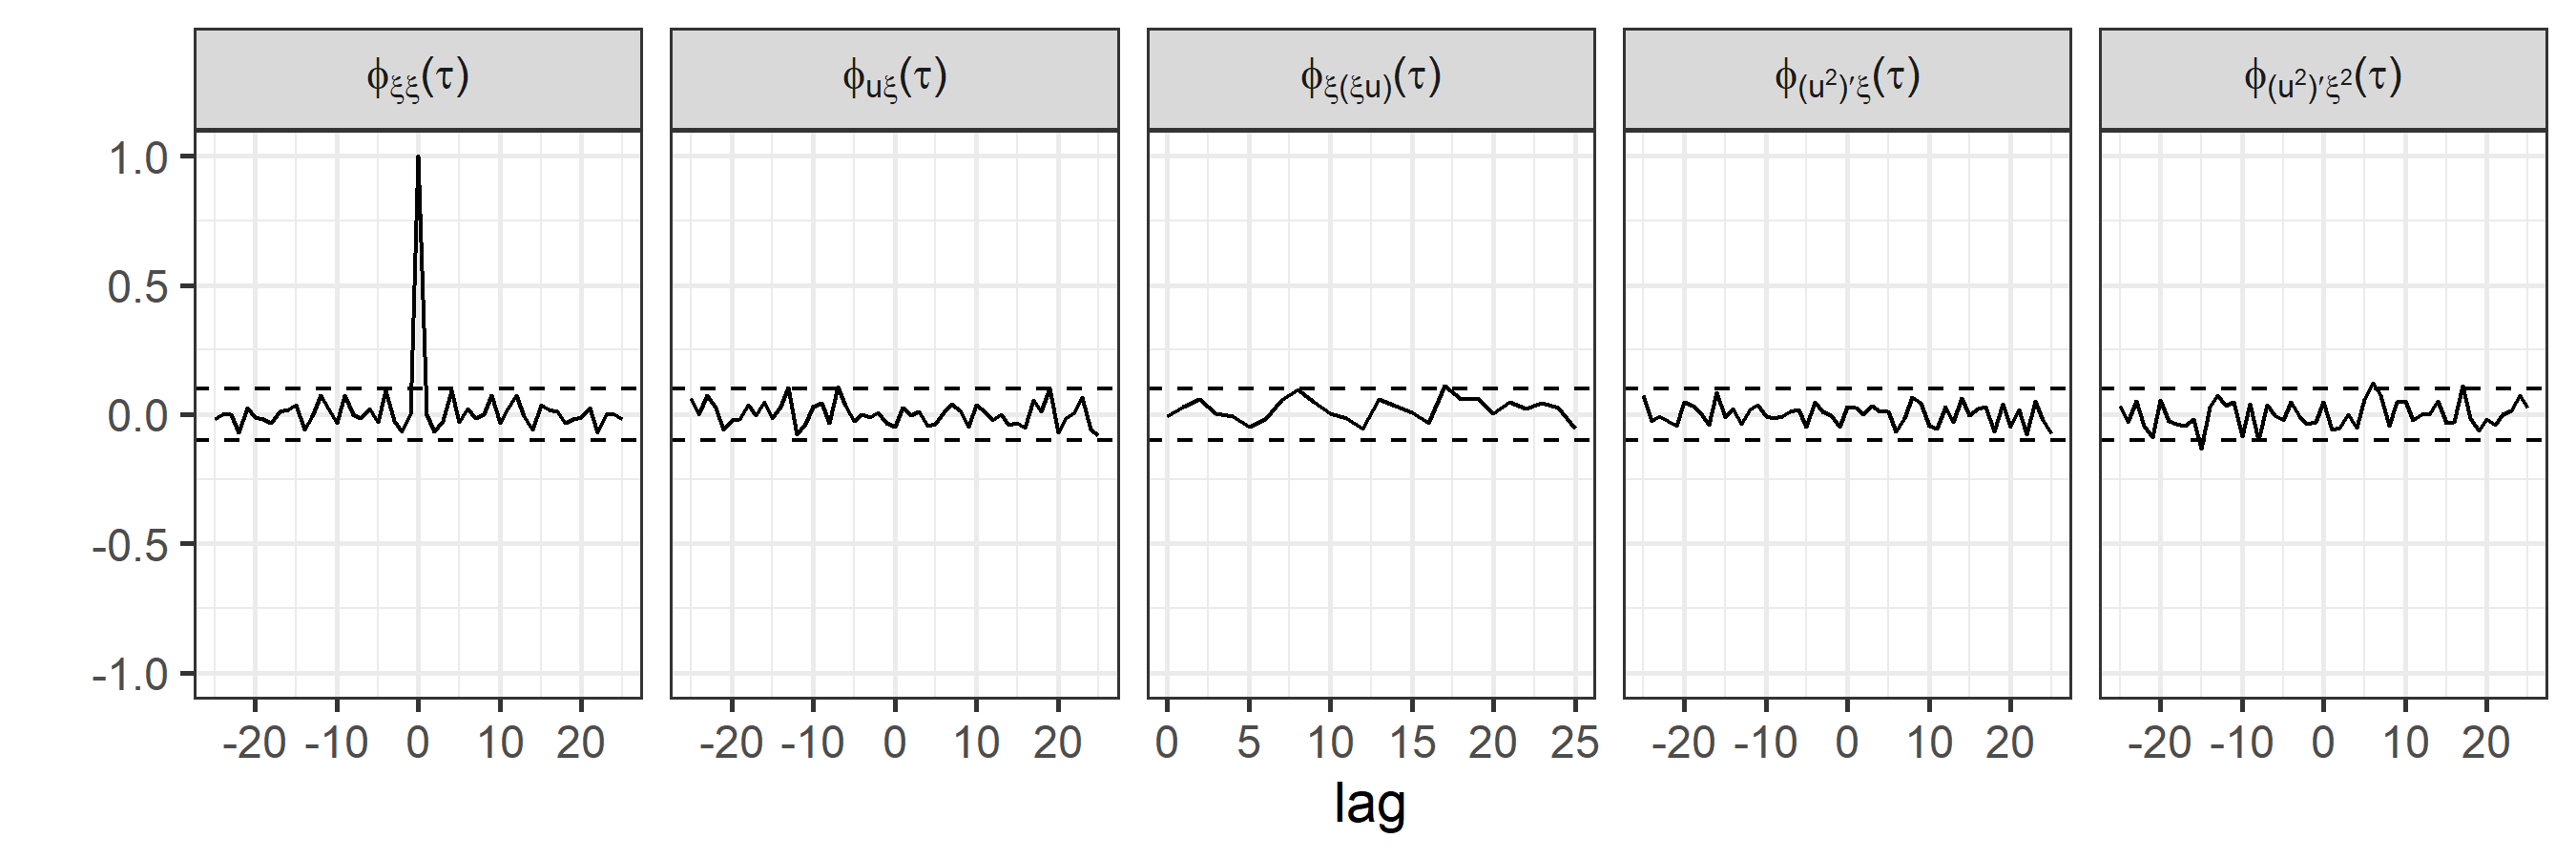
\includegraphics[width=15cm,keepaspectratio]{ex1xcorrel}
	\caption{Statistical analysis of the residuals for Example 1. It is possible to see that the tests are adequately satisfied.}
	\label{fig:ex1xcorrel}
	
	% ATTENTION ATTENTION ATTENTION ATTENTION ATTENTION ATTENTION ATTENTION ATTENTION ATTENTION
	% ATTENTION ATTENTION ATTENTION ATTENTION ATTENTION ATTENTION ATTENTION ATTENTION ATTENTION
	% ATTENTION ATTENTION ATTENTION ATTENTION ATTENTION ATTENTION ATTENTION ATTENTION ATTENTION
	% ATTENTION ATTENTION ATTENTION ATTENTION ATTENTION ATTENTION ATTENTION ATTENTION ATTENTION
	% ATTENTION ATTENTION ATTENTION ATTENTION ATTENTION ATTENTION ATTENTION ATTENTION ATTENTION
	
	% CODE TO GENERATE FIGURES
	
	% ggsave("D:/Google Drive/Trabalho/Publicacoes/2018 JSS - narmax toolbox/paper/fig/ex2e.png", width=9, height=3)
	
	% ATTENTION ATTENTION ATTENTION ATTENTION ATTENTION ATTENTION ATTENTION ATTENTION ATTENTION
	% ATTENTION ATTENTION ATTENTION ATTENTION ATTENTION ATTENTION ATTENTION ATTENTION ATTENTION
	% ATTENTION ATTENTION ATTENTION ATTENTION ATTENTION ATTENTION ATTENTION ATTENTION ATTENTION
	% ATTENTION ATTENTION ATTENTION ATTENTION ATTENTION ATTENTION ATTENTION ATTENTION ATTENTION
	% ATTENTION ATTENTION ATTENTION ATTENTION ATTENTION ATTENTION ATTENTION ATTENTION ATTENTION
	
\end{figure}

The input argument for \verb|predict()| that controls which type of prediction (OSA or FR) is \verb|K|, where 0 and 1 set FR and OSA predictions respectively. In the examples given here the output for the predictions nomenclature also follow the same convention (\verb|P0| and \verb|P1|). The performance of the prediction in terms of $ R^2 $ is given right below each function call for prediction. The correlation based tests can be plotted by simply typing \verb|R> P1$xcorrel|, and the output is given in Figure~\ref{fig:ex1xcorrel}. 

\section{Example 2: heating system}

The present case study is a heating system whose data is available at the DaISy (Database for the Identification of Systems) \cite{Moor2019}. The input commands a 300 Watt lamp suspended above a steel plate whose temperature is the output measured. This case study has been used in \cite{Dullerud96} for the model validation.

First we read the data and divide the dataset for estimation and validation. In this example we have 801 samples, so we use the first 400 samples (stored in \verb|ye,ue|)) to construct the model and the rest to validate it.

\begin{verbatim}
R> data <- matrix(scan("../data/heating_system.dat"),
nrow=801,byrow=TRUE)
R> u <- data[,2]
R> y <- data[,3]
R> ye <- y[1:400]
R> ue <- u[1:400]
\end{verbatim}

Now we define the model order as

\begin{verbatim}
R> mdl <- armax(ny= 4,nu = 4,ne = 10)
armax(ny = 4, nu = 4, ne = 10)

Not estimated
\end{verbatim}

and estimate its parameters through

\begin{verbatim}
R> mdl <- estimate(mdl,ye,ue)
R> print(mdl)
armax(ny = 4, nu = 4, ne = 10)

Term         Coefficient
-y(k-1)             -1.8730
-y(k-2)              0.5438
-y(k-3)              0.6032
-y(k-4)             -0.2732
u(k-1)              0.0939
u(k-2)              0.2126
u(k-3)              0.0013
u(k-4)             -0.2892
e(k-1)             -0.6480
e(k-2)             -0.4008
e(k-3)              0.0202
e(k-4)              0.0927
e(k-5)             -0.0467
e(k-6)              0.0547
e(k-7)              0.0595
e(k-8)             -0.0811
e(k-9)             -0.0386
e(k-10)              0.1087
\end{verbatim}

We have increased the model order until the correlation based tests in were satisfied. All the information related to the predictions can be obtained by 

\begin{verbatim}
R> Pe1 <- predict(mdl, ye, ue, K = 1) # one-step-ahead
Running armax prediction ... 
Done. R2 = 1.0000
R> Pa0 <- predict(mdl, y, u, K = 0)   # free-run
Running armax prediction ... 
Done. R2 = 0.9904          
\end{verbatim}

Then the plot of the residuals, prediction versus measured data, and correlation-based tests can be obtained respectively by the code below. The command for checking the predictions is depicted below and in Figure~\ref{fig:ex2a}.

\begin{verbatim}
R> Pa0$ploty
\end{verbatim}

\begin{figure}[h!]
	\centering
	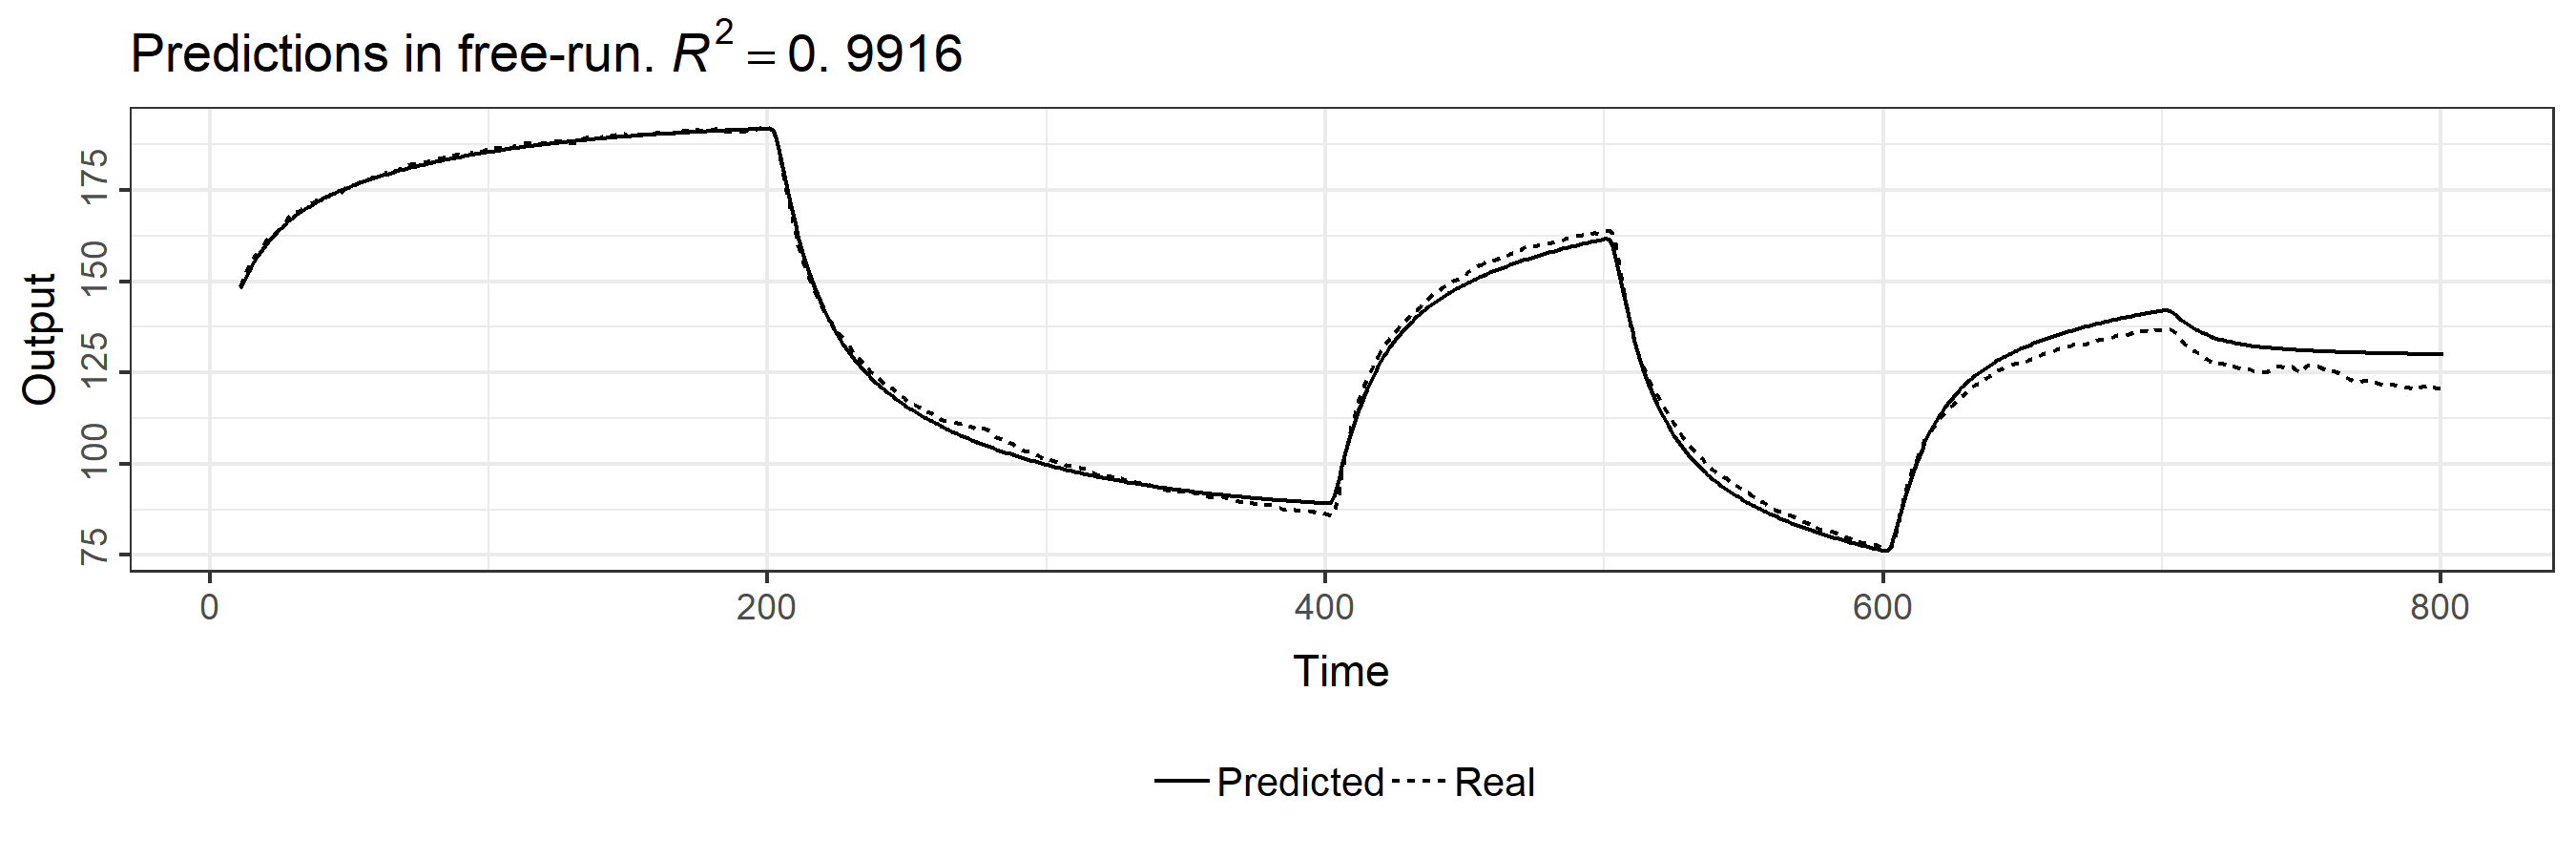
\includegraphics[width=15cm,keepaspectratio]{ex2y}
	\caption{Predictions in FR simulation for all measured data for the model created in Example 2. It is possible to see that the predictions yield a reasonable $ R^2 $.} \label{fig:ex2a}
\end{figure}

The error can also be plotted accordingly, by issuing the following line.

\begin{verbatim}
R> Pa0$plote  
\end{verbatim}

The output is shown in Figure~\ref{fig:ex2b} shows. We can see that the error increases in the validation phase (last 400 samples). 

\begin{figure}[h!]
	\centering
	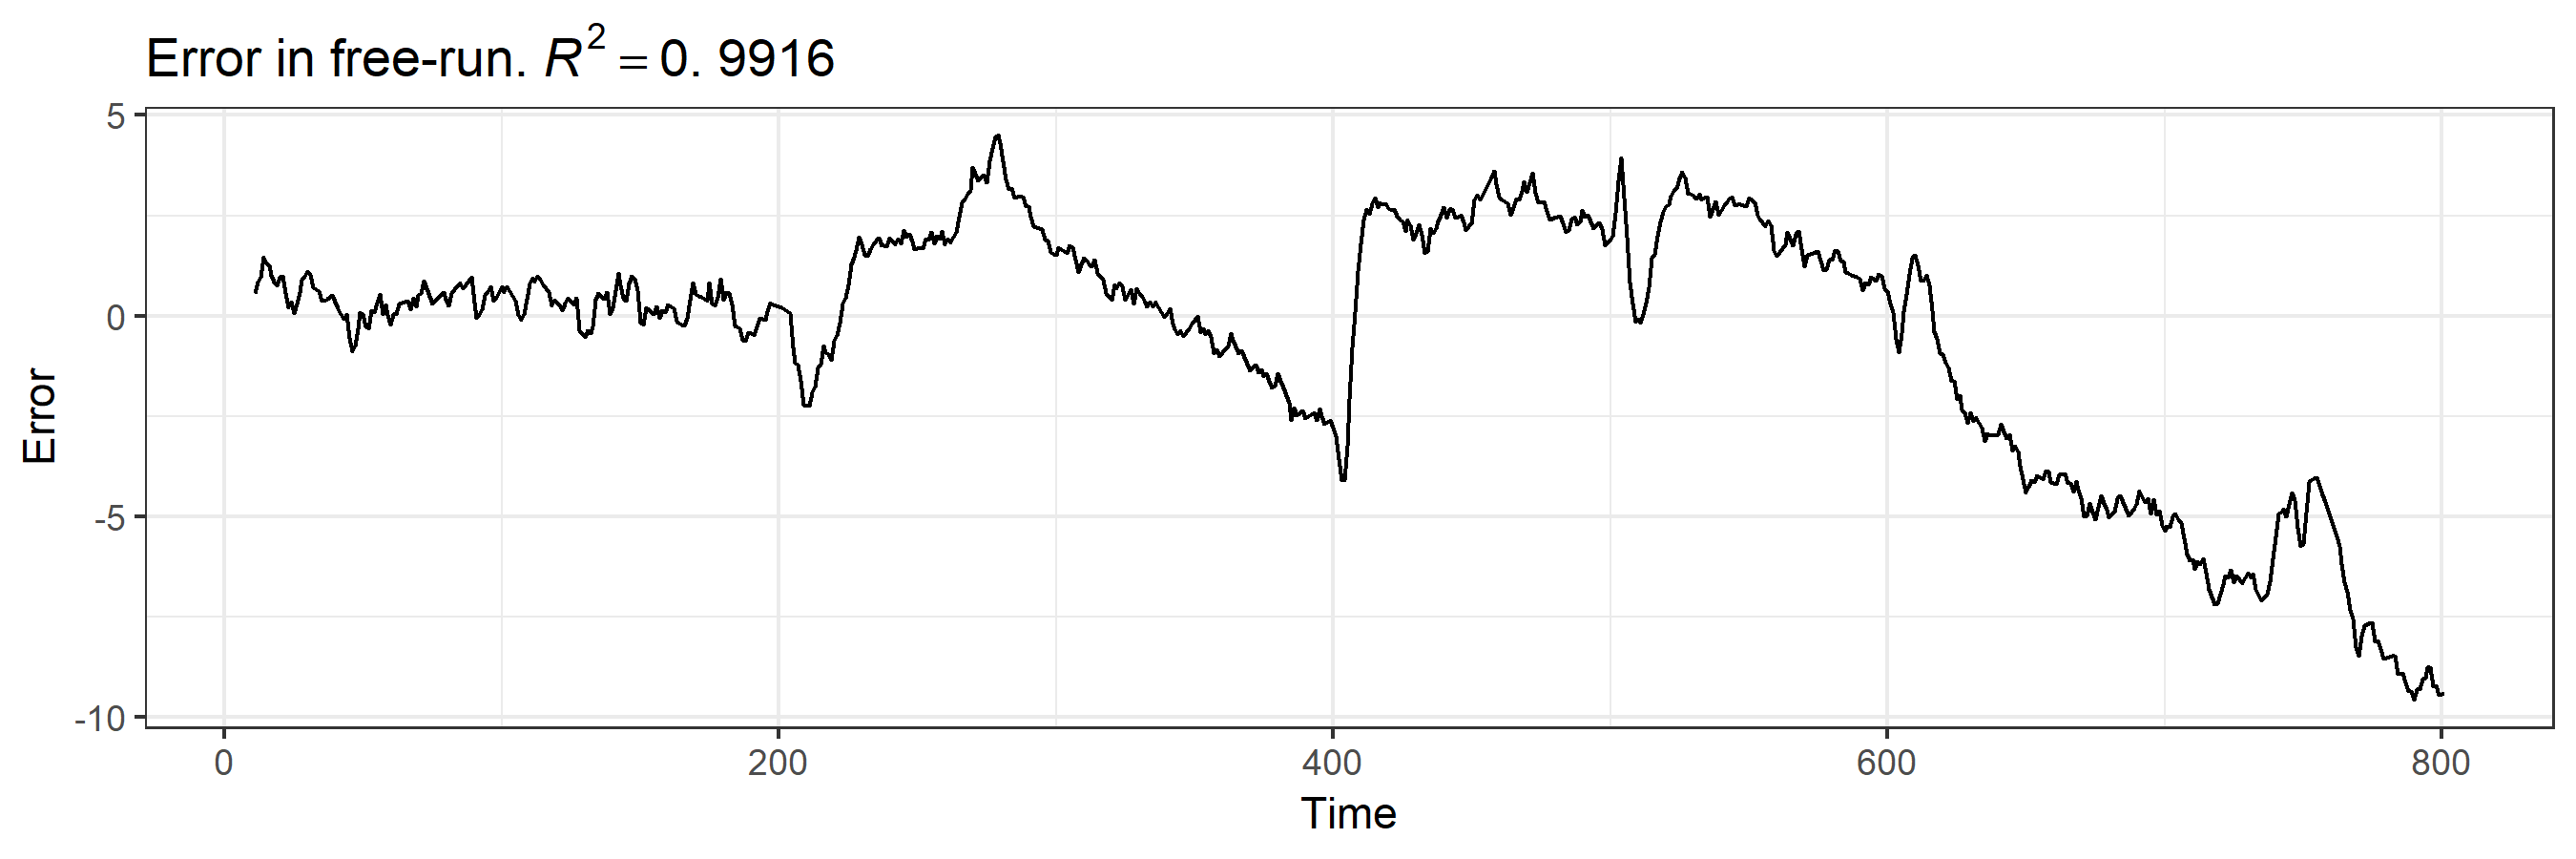
\includegraphics[width=15cm,keepaspectratio]{ex2e}
	\caption{Errors in FR simulation the model created in Example 2.} \label{fig:ex2b}
\end{figure}

The correlation tests can be issued by the command below. They confirm that the model is valid as the statistical analysis shows in Figure~\ref{fig:ex2c}. In this example we have increased the model orders until the tests were satisfied. The results of the tests indicate that the dynamics present in this set of measurements has been adequately captured by the model.
\begin{verbatim}
R> Pe1$xcorrel 	
\end{verbatim}

\begin{figure}[h!]
	\centering
	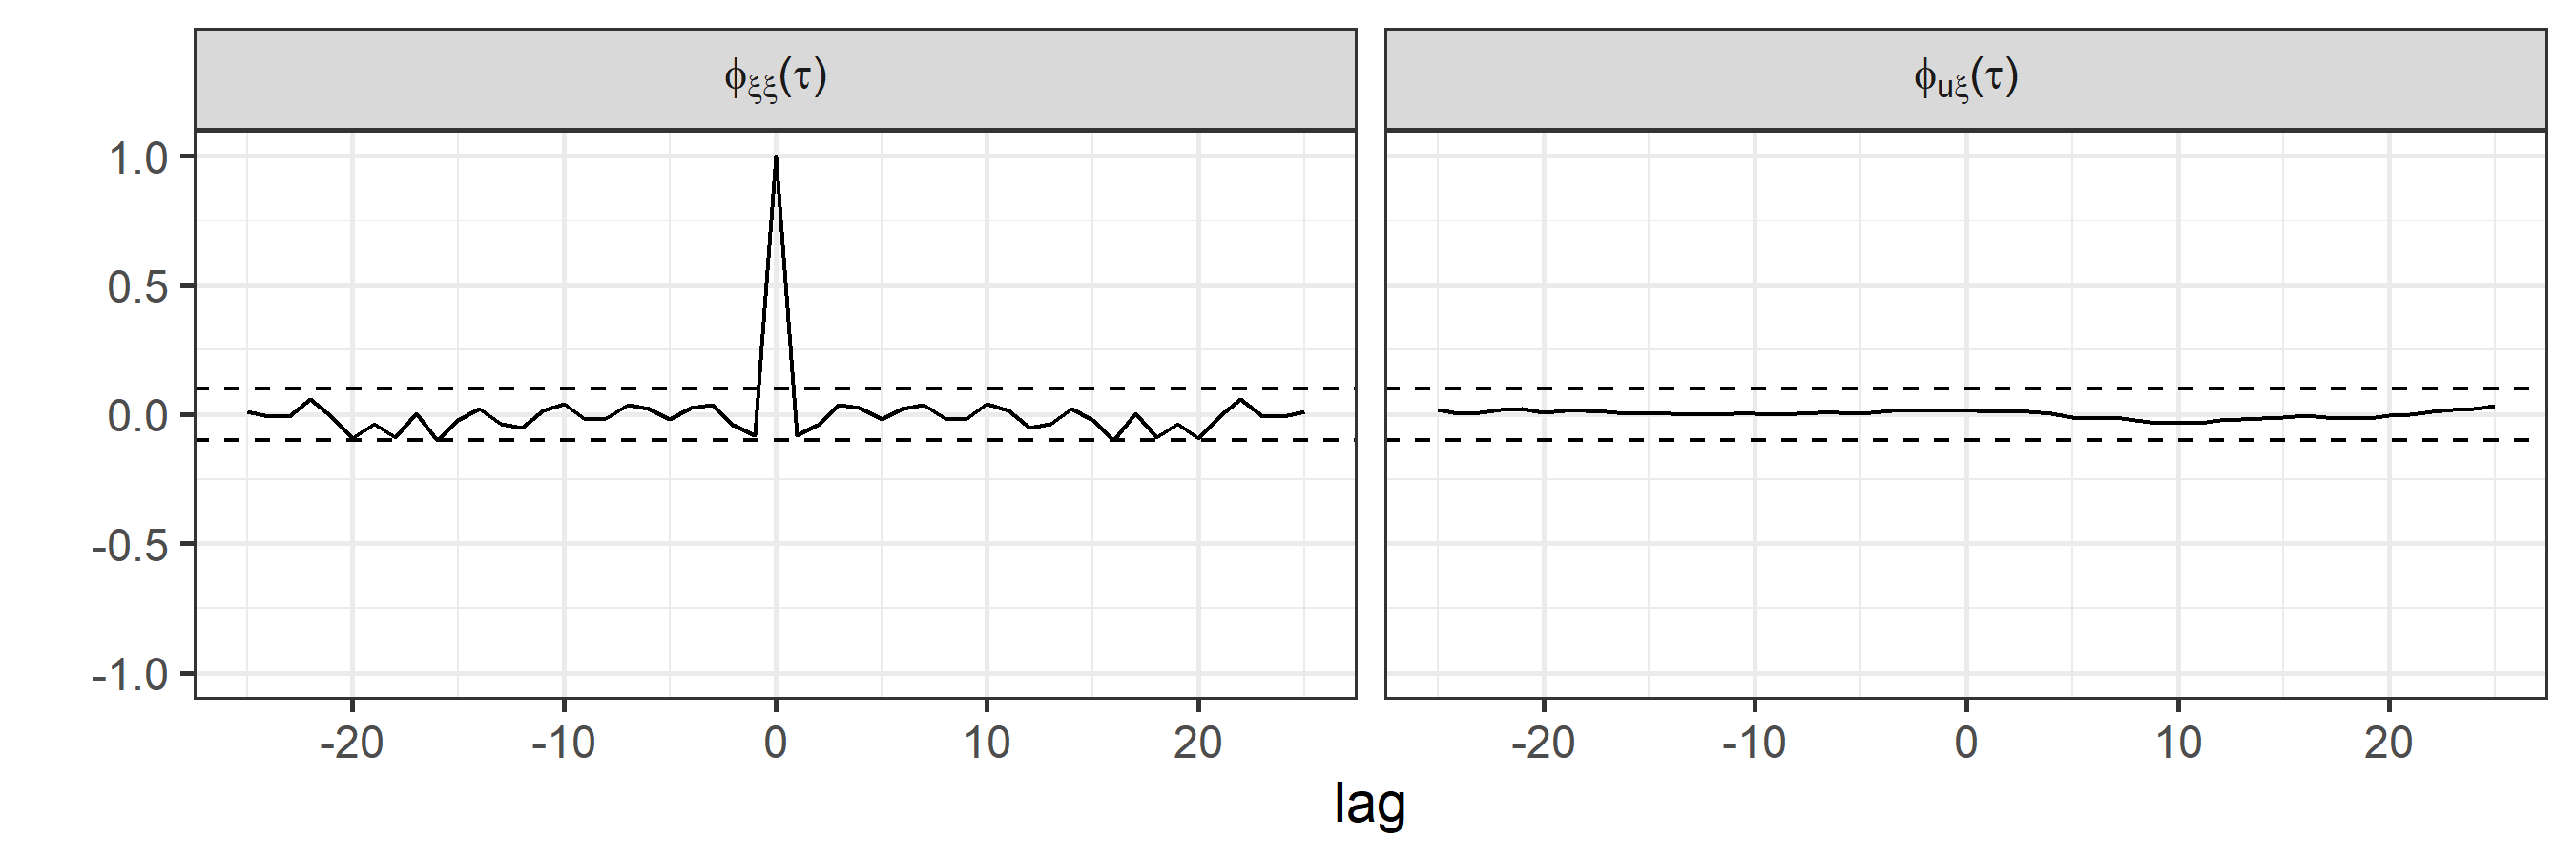
\includegraphics[width=15cm,keepaspectratio]{ex2xc}
	\caption{Correlation tests in Equation~\ref{eq:xcorr} in the linear systems case for the model created in Example 2. The order of the noise terms were increased until the tests in (c) were satisfied.} \label{fig:ex2c}
\end{figure}

\section{Example 3: Box-Jenkins gas furnace}

This example has been extensively used in the nonlinear identification literature for testing new methods, see e.g. \cite{Sugeno93}, \cite{AYALA2016378}. The input is the gas flow rate in a gas furnace, whose CO2 concentration in the outlet is the measured desired output. The first step here is to read the data and separate its part used for estimation. The whole dataset contains 296 samples, and we use the first 250 for estimation.

\begin{verbatim}
R> u <- scan("../data/ts22.dat")
R> y <- scan("../data/ts23.dat")
R> ye <- y[1:250]
R> ue <- u[1:250]
\end{verbatim}

Now we test two model structures. To do so, we create two variables that contain each of them as below.

\begin{verbatim}
R> mdl1 <- narmax(ny = 1, nu = 1, ne = 1, nl = 2)
R> mdl2 <- narmax(ny = 5, nu = 5, ne = 1, nl = 2)
\end{verbatim}

The estimation is performed using the \verb|estimate()| function, as follows.

\begin{verbatim}
R> mdl1 <- estimate(mdl1, ye, ue, rho_p = 1e-5, rho_n = 1e-6)
R> mdl2 <- estimate(mdl2, ye, ue, rho_p = 1e-5, rho_n = 1e-6)
\end{verbatim}

Now we can run the model predictions in OSA and FR for each model. We do this for the estimation and all dataset, respectively, as below.

\begin{verbatim}
R> Pe1 <- predict(mdl1, ye, ue, K = 1)
Running narmax prediction ... 
Done. R2 = 0.9859      
R> Pa1 <- predict(mdl1, y,  u,  K = 0)
Running narmax prediction ... 
Done. R2 = 0.8174     
R> Pe2 <- predict(mdl2, ye, ue, K = 1)
Running narmax prediction ... 
Done. R2 = 0.9977                     
R> Pa2 <- predict(mdl2, y,  u,  K = 0)
Running narmax prediction ... 
Done. R2 = 0.9312        
\end{verbatim}

We can see that, while the performance in OSA is very similar for both models, the first model performs poorly in FR. The plots for both models in FR are shown in Figure~\ref{fig:ex3y} and we obtain them by running the following code.

\begin{verbatim}
R> Pa1$ploty
R> Pa2$ploty
\end{verbatim}

\begin{figure}[t!]
	\centering
	\begin{tabular}{c}
		(a) \\
		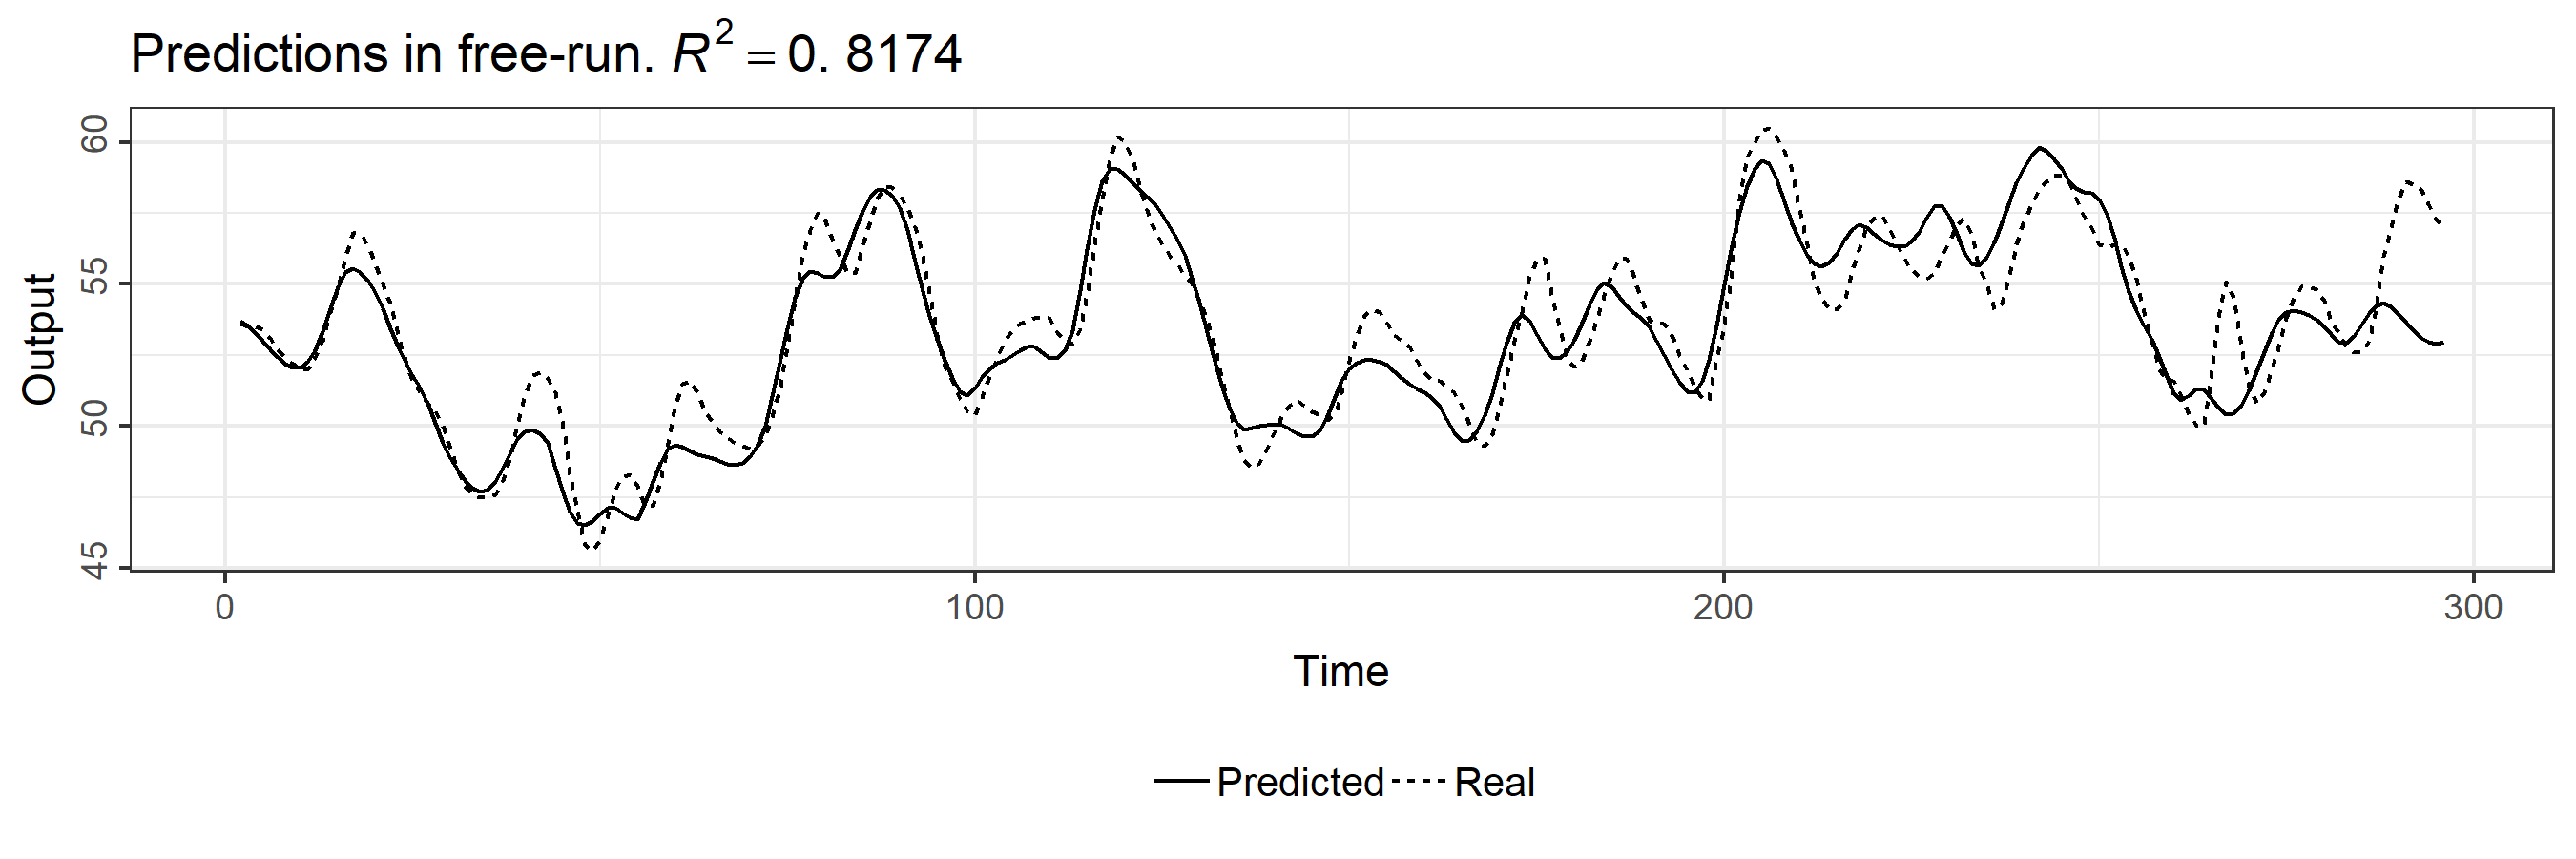
\includegraphics[width=15cm,keepaspectratio]{ex3y1}  \\ 
		(b) \\
		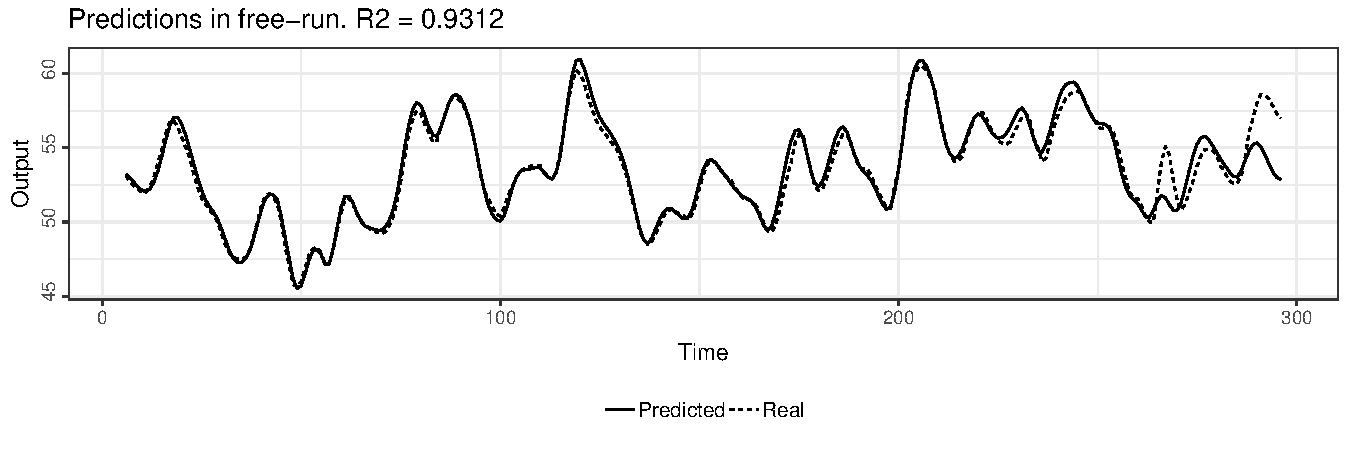
\includegraphics[width=15cm,keepaspectratio]{ex3y2}
	\end{tabular}
	\caption{Predictions in FR for the models created in Example 3. (a) mdl1 and (b) mdl2. It is possible to confirm that by increasing the model orders the prediction was improved.} \label{fig:ex3y}
\end{figure}

The correlation-based tests also reveal that mdl1 fails to capture the dynamics present in the dataset. We obtain the plot for both models as shown in the code below. Again, by increasing the orders of the model we improved the model validation metrics as depicted in Figure~\ref{fig:ex3xc}.

\begin{figure}[t!]
	\centering
	\begin{tabular}{c}
		(a) \\
		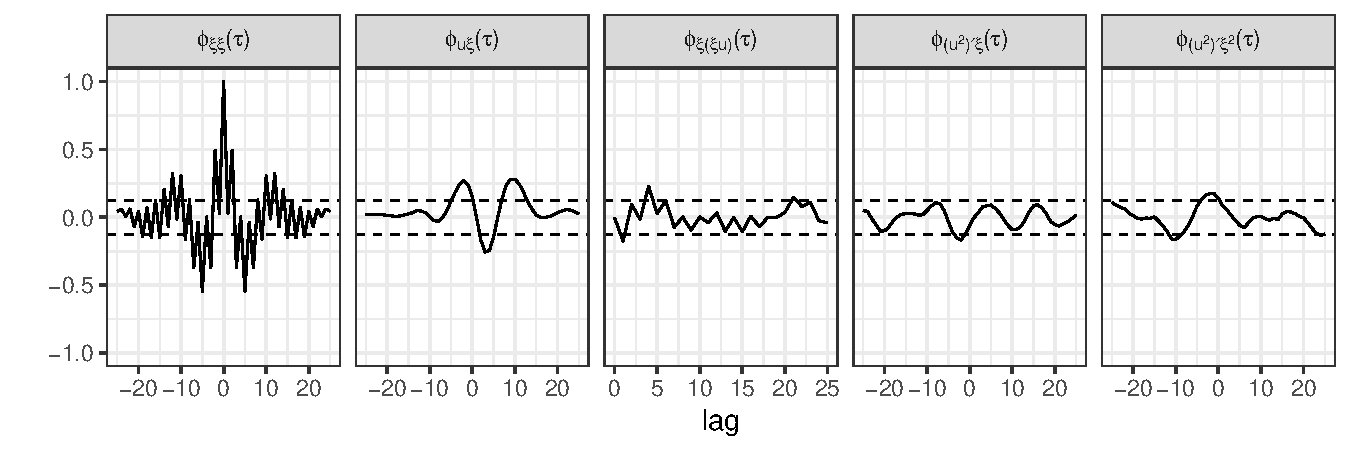
\includegraphics[width=15cm,keepaspectratio]{ex3xc1}  \\ 
		(b) \\
		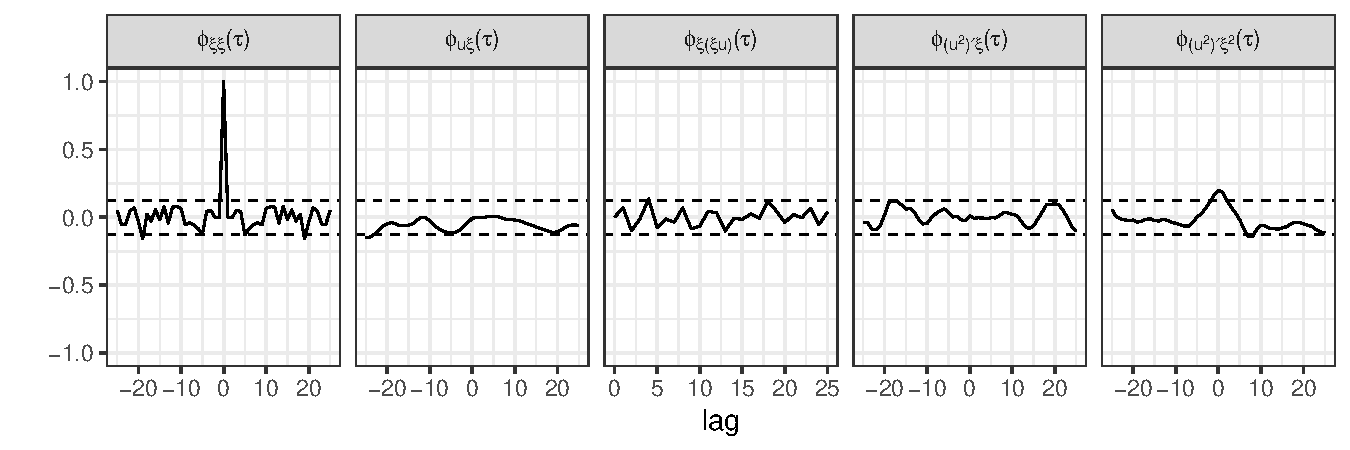
\includegraphics[width=15cm,keepaspectratio]{ex3xc2}
	\end{tabular}
	\caption{Statistical analysis of the residuals for the models created in Example 3 - Box-Jenkins gas furnace. (a) mdl1 and (b) mdl2. Increasing the complexity of the model improved the requirements given by the correlation-based tests.} \label{fig:ex3xc}
\end{figure}



\section{Example 4: Coupled Drives}

The coupled drives system is equipped by two motors connected by a flexible belt and a pulley fixed by a spring. The benchmark was introduced by \cite{Wigren2013} and as the data is freely available in the internet it has been increasingly used to test new identification algorithms, see e.g. \cite{Sabahi2016}, \cite{Wachel2017}. Both motors are actuated with the same input and the velocity is measured as the output with a sensor insensitive to the direction of the movement. The firs step is to load the data and define a NARMAX model with a suitable order. After some trial and error, we get the following model structure and ELS-FROLS estimation parameters.

\begin{verbatim}
R> data <- read.csv('../data/DATAUNIF.csv',stringsAsFactors=FALSE,header = TRUE)
R> u <- data$u12
R> y <- data$z12
R> mdl <- narmax(ny = 10, nu = 10, ne = 2, nl = 2)
R> mdl <- estimate(mdl, y, u, rho_p = 1e-3, rho_n = 1e-5)
\end{verbatim}

Now that the model has been created, we can check the predictions, as done below. 

\begin{verbatim}
R> P1 <- predict(mdl, y, u, K = 1)
Running narmax prediction ... 
Done. R2 = 0.9986           
R> P0 <- predict(mdl, y, u, K = 0)
Running narmax prediction ... 
Done. R2 = 0.9590    
\end{verbatim}

Again the plots for the predictions and the correlation-based tests can be shown with the following commands. The outputs generated are presented in Figure~\ref{fig:ex4}.

\begin{verbatim}
R> P0$ploty
R> P1$xcorrel
\end{verbatim}

\begin{figure}[t!]
	\centering
	\begin{tabular}{c}
		(a) \\
		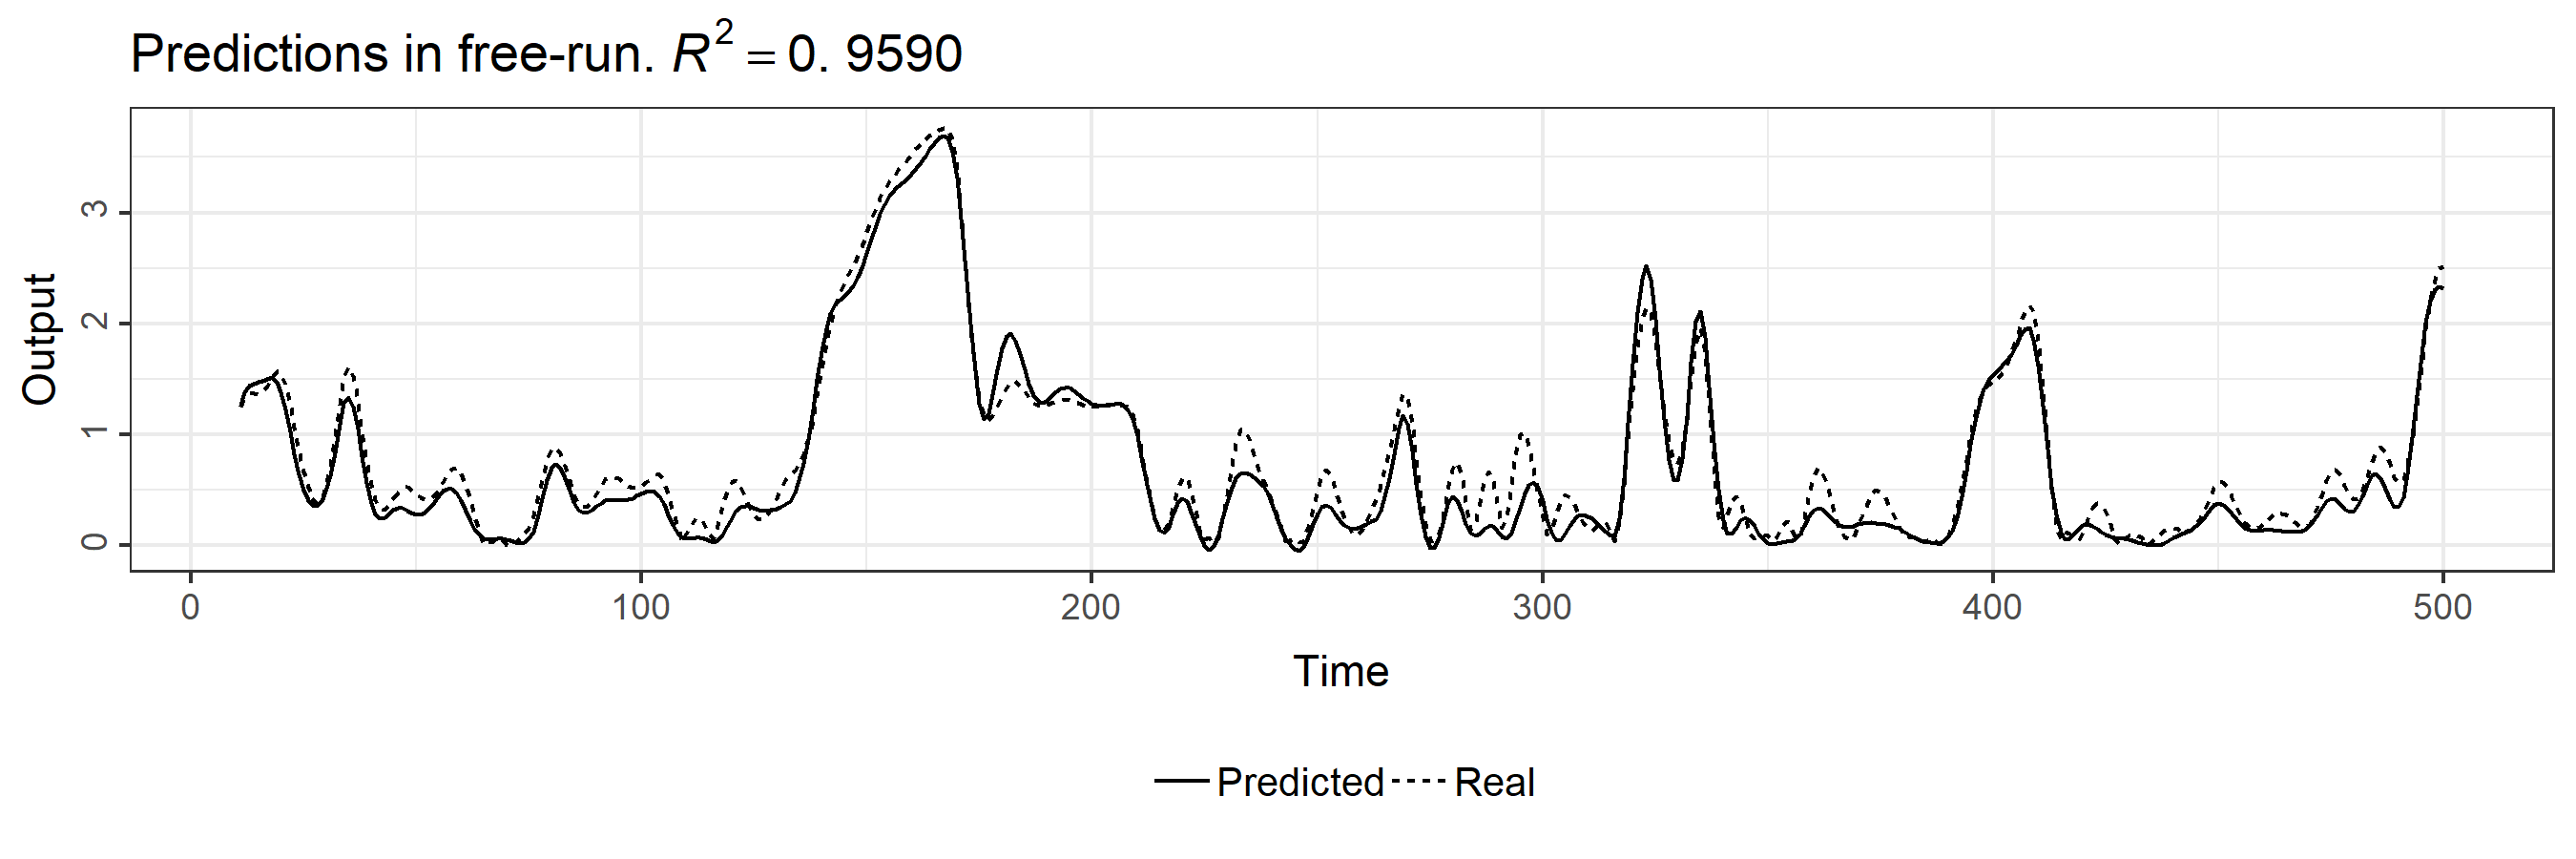
\includegraphics[width=15cm,keepaspectratio]{ex4y}  \\ 
		(b) \\
		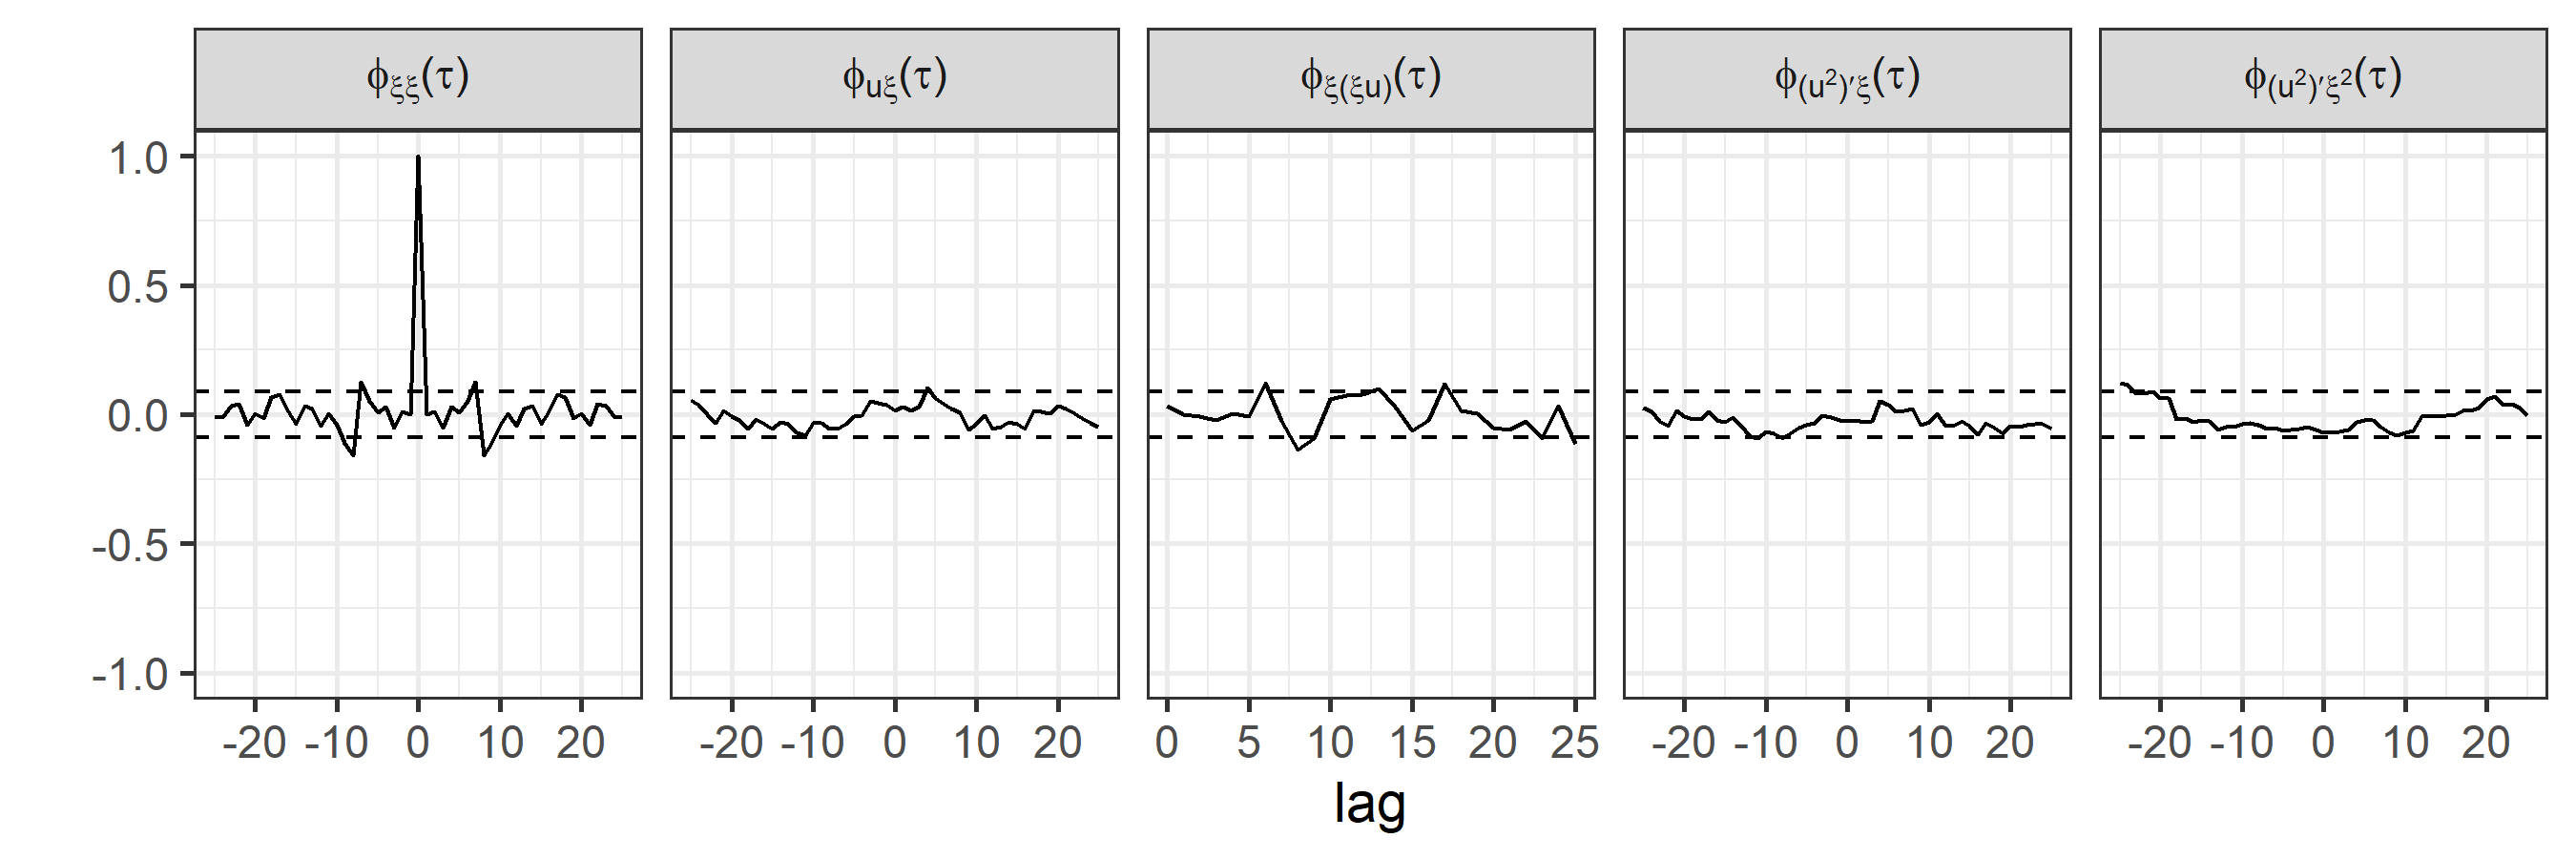
\includegraphics[width=15cm,keepaspectratio]{ex4xc}
	\end{tabular}
	\caption{Outputs for the model created in Example 4 - coupled drives exchanger: (a) predictions in FR simulation for all measured data and (b) the correlation tests in Equation~\ref{eq:xcorr}. We can see here that in spite that the predictions are accurate in FR, it is still possible to improve the model with the same dataset, as the few excursions in the first test show.} \label{fig:ex4}
\end{figure}

\bibliographystyle{elsarticle-num} 
\bibliography{refs}

%% The Appendices part is started with the command \appendix;
%% appendix sections are then done as normal sections
%% \appendix

%% \section{}
%% \label{}

%% References:
%% If you have bibdatabase file and want bibtex to generate the
%% bibitems, please use
%%
%%  \bibliographystyle{elsarticle-num} 
%%  \bibliography{<your bibdatabase>}

%% else use the following coding to input the bibitems directly in the
%% TeX file.

\end{document}
\endinput
%%
%% End of file `SoftwareX_article_template.tex'.
